\chapter{High Level Design}
Our implementation required 8 \texttt{GAL22V10} chips. 6 of these chips were
MOD-n counters which were modified to suit the purpose of providing particular
traffic flows and their timings. The remaining 2 were overarching control chips
to provide inter-flow logic based on sensor inputs and current flow state. A
basic diagram is provided in figure \ref{fig:overall-design}. The diagram does
not explain everything in the design,those more complex details are provider
later on in the document. The ``Minor Controller'' was necessary due to a
limitation in the number of inputs in the main controller. This diagram does not
indicate anything to do with pin positions, rather, it shows the conceptual
blocks of the design. Controller outputs are indicated in red, and Controller
inputs are indicated in green. Flow chip colours are vice-versa.  

\begin{figure}
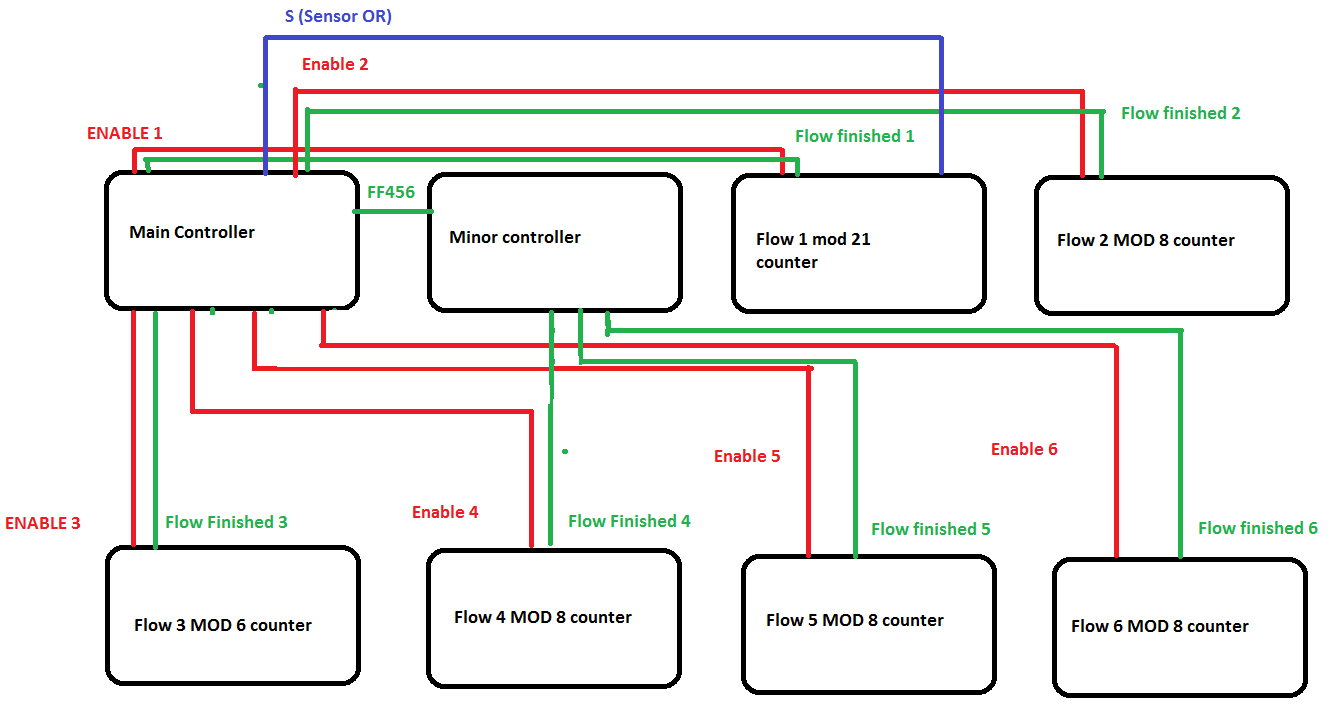
\includegraphics[width=\linewidth]{img/LJNpzV.png}
\label{fig:overall-design}
\end{figure}